\section{Introduction}

The inverse folding problem in RNA design addresses a fundamental computational challenge: determining which nucleotide sequence will reliably fold into a specified three-dimensional backbone structure \citep{tang2024survey,tan2025r3design}. This problem represents the cornerstone of rational RNA engineering \citep{wong2024deep}, enabling systematic design of functional molecules for gene regulation \citep{green2014toehold}, therapeutics \citep{yip2024therapeutic}, and synthetic biology applications \citep{pfeifer2023harnessing}.

{
\emph{Designability}—defined as the total number or density of sequences that fold into a specific target structure—is a critical property for functional RNA. Highly designable structures are easier to discover, more mutation-robust \citep{england2003naturalselectdesignablefold}, and tend to inhabit thermodynamically favorable \emph{designable basins} (regions in sequence space with a high density of valid solutions) \citep{designability_li_1996}. Optimizing geometry alone may reach thin, fragile ridges in sequence space; coupling geometry with ensemble stability biases search toward these robust basins \citep{schuster1994rna2dshape}.
}

Contemporary geometric neural networks have achieved significant progress on this task \citep{wu2023integration,wu2023hierarchical,liu2025sentences,patil2024towards}. Models such as gRNAde \citep{joshi2025grnade} utilize graph neural networks with geometric vector perceptrons to capture spatial relationships within RNA tertiary structures, delivering impressive sequence recovery performance across benchmark datasets. 
{ However, unlike proteins that maintain relatively stable native folds, RNA molecules exhibit inherent conformational flexibility that causes them to sample multiple competing structures in solution \citep{ganser2019roles, zadeh2011nucleic}.}

Current inverse folding methods \citep{Hou2025ridiffusion, wong2024deep}, when optimized for sequence similarity or a single structural proxy, often neglect \emph{designability} and thermodynamic stability, and therefore \emph{do not} consistently adopt the intended conformation under physiological conditions.

Prevailing evaluations emphasize geometric correspondence (e.g., TMscore \citep{zhang2004tmscore} and RMSD for global alignment, pLDDT \citep{jumper2021alphafold2} for local fidelity), but these alone provide limited insight into \emph{ensemble viability} and \emph{designability}. As a result, sequences can score well structurally yet occupy narrow, unstable basins that admit competing conformations in solution \citep{bernard2024rnadvisor}. This evaluation-centric limitation produces sequences that achieve excellent structural scores while exhibiting poor ensemble behavior, sampling multiple competing conformations, and failing to demonstrate practical utility in biological applications \citep{zhou2023rna}. From a design perspective, single-objective optimization cannot fully address the multifaceted challenges inherent to RNA structural stability, where geometric fidelity must be balanced against thermodynamic preferences and conformational robustness.

\begin{figure}[!t] 
    \centering 
    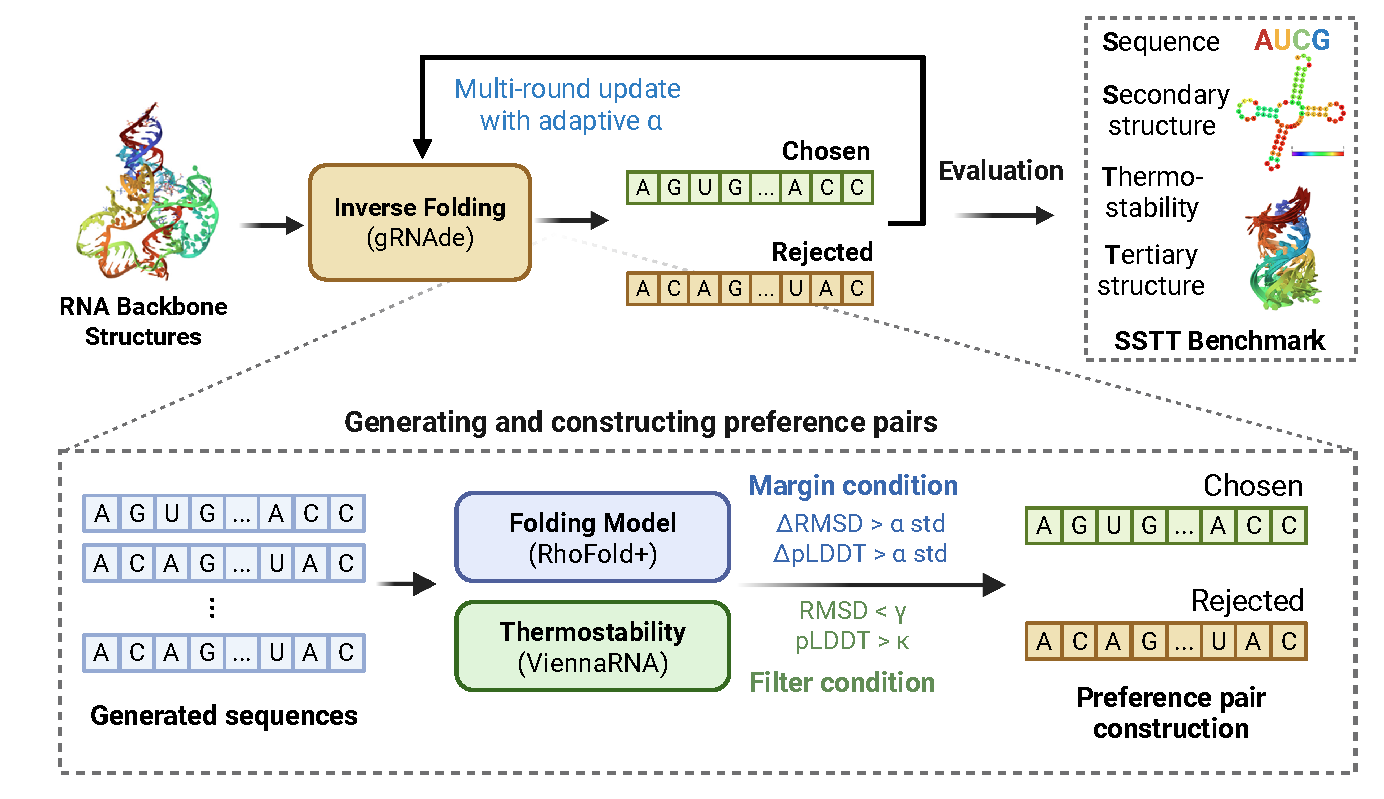
\includegraphics[width=0.9\textwidth]{figs/Main.pdf} 
    \vspace{-1em}
    \caption{Overview of RiboPO framework.} 
    \label{fig:main} 
\end{figure}

To address these limitations, we present \textbf{RiboPO}, a reinforcement-learning–from–physical-feedback framework for RNA tertiary inverse folding that \emph{explicitly} incorporates thermodynamic stability alongside geometry. Our approach reframes RNA inverse folding as a multi-objective preference optimization problem, representing a paradigm shift from purely geometric to biophysically-informed design. Unlike previous RL applications limited to RNA secondary structure prediction, RiboPO operates on full tertiary structures while balancing structural accuracy with thermodynamic stability.
Our contributions are threefold:
\begin{itemize}[leftmargin=*]
\item  We incorporate thermodynamic stability measures into the reward for RNA inverse folding, representing the first systematic approach to include ensemble stability properties that existing RNA design methods have consistently overlooked.
Our framework employs offline RL with precomputed training pairs, enabling efficient use of costly biophysical calculations during training.
\item Second, our multi-objective preference optimization framework enables iterative refinement across competing design objectives through successive training rounds. This approach allows dynamic balancing between structural fidelity, local interaction accuracy, and thermodynamic stability without requiring online structure prediction during training.
\item Third, we establish the \textbf{SSTT Benchmark} (\textbf{S}equence, \textbf{S}econdary, \textbf{T}ertiary, \textbf{T}hermostability) for comprehensive evaluation of RNA sequence generation quality. Our analysis reveals fundamental limitations in current geometric-only approaches and demonstrates that preference-based optimization significantly improves both designability and thermodynamic stability while maintaining competitive sequence recovery performance.
\end{itemize}

On the DAS split \citep{das2010farfar, joshi2025grnade} with our comprehensive SSTT suite, RiboPO achieves \emph{general} improvements across dimensions: secondary-structure self-consistency (EternaFold scMCC: $+0.12$, \textbf{+20\%}; $0.72$ vs.\ $0.60$) and thermostability (MFE: \textbf{$-4.03$}~kcal/mol, \textbf{12.3\%}; $-36.86$ vs.\ $-32.83$), while maintaining competitive recovery and strong tertiary fidelity (RMSD \textbf{10.23}\AA\ vs.\ 10.66\AA; \%RMSD$\le 8$\AA: \textbf{0.51} vs.\ 0.46). 
{ In Appendix \ref{subsec:pareto} (Pareto Analysis), we show that these shifts correspond to movement into more \emph{designable basins} (lower energy, higher structural consistency).} 
In \S\ref{sec:experiments} (Ablations), we validate the necessity of (i) variability-aware pair construction, (ii) DPO+$\lambda_{\text{SFT}}$ loss, and (iii) the multi-round schedule. Practically, sampling efficiency improves substantially.

Overall, preference-based optimization with physical feedback yields sequences that are not only structurally accurate but also ensemble-robust—advancing RNA design toward practically viable, mutation-tolerant solutions.